\documentclass[journal]{IEEEtran}
\hyphenation{op-tical net-works semi-conduc-tor}
\usepackage{graphicx}



\begin{document}

\title{Machine learning based football outcome prediction and visualization}


\author{Devam~Trivedi,
        Umang~Raval,
        and~Kisore~S% <-this % stops a space
}



\markboth{SCOPE school}%
{Shell \MakeLowercase{\textit{et al.}}: Bare Demo of IEEEtran.cls for Journals}

\maketitle

\begin{abstract}
  Football is a worldwide game, with 100s of major and
  minor leagues. This paper aims for the visualization of
  football teams considering different aspects and
  comparing different teams and players through
  successive seasons, thereby showing their evolution
  throughout the years and to showcase the
  consistency of a player, fixtures in a league,
  along with the win/loss percentage of different teams
  using various machine learning techniques like Logistic
  Regression, Naive Bayes and Support Vector Machine algorithms.
\end{abstract}

% Note that keywords are not normally used for peerreview papers.
\begin{IEEEkeywords}
  Football prediction, visualization
\end{IEEEkeywords}

\IEEEpeerreviewmaketitle



\section{Introduction}
\IEEEPARstart{F}{ootball} is the most popular sport in the world. According to a FIFA survey, about 256 million people i.e. 4\% of the world population are actively involved in playing or just the following soccer. With about 20,000 professional players. Every year, hundreds of leagues are played, each consisting of hundreds of games. Some of these leagues are watched by millions of fans around the world. This vast amount of games played results in a huge amount of data. As a consequence, it is often hard to remember how a team performed last year, let alone five years ago and it can sometimes be difficult to keep track of all the football leagues and player statistics. 

This information is often openly available, but hard to find. Furthermore, different seasons are rarely compared to each other or visualized together. This could be useful though, to see the evolution of a certain team, an individual player or a set of teams throughout the years.

Apart from that analysts and coaches in soccer sports need to investigate large sets of past matches of opposing teams in a short time to prepare their teams for upcoming matches. Thus, they need appropriate methods and systems supporting them in searching for soccer moves for comparison and explanation.
\begin{figure}
  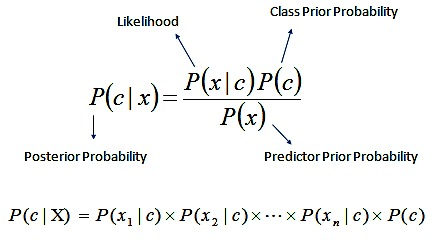
\includegraphics[width=\linewidth]{naive-bayes.jpeg}
  \caption{Naive bayes algorithm}
  \label{fig:algo1}
\end{figure}

\begin{figure}
  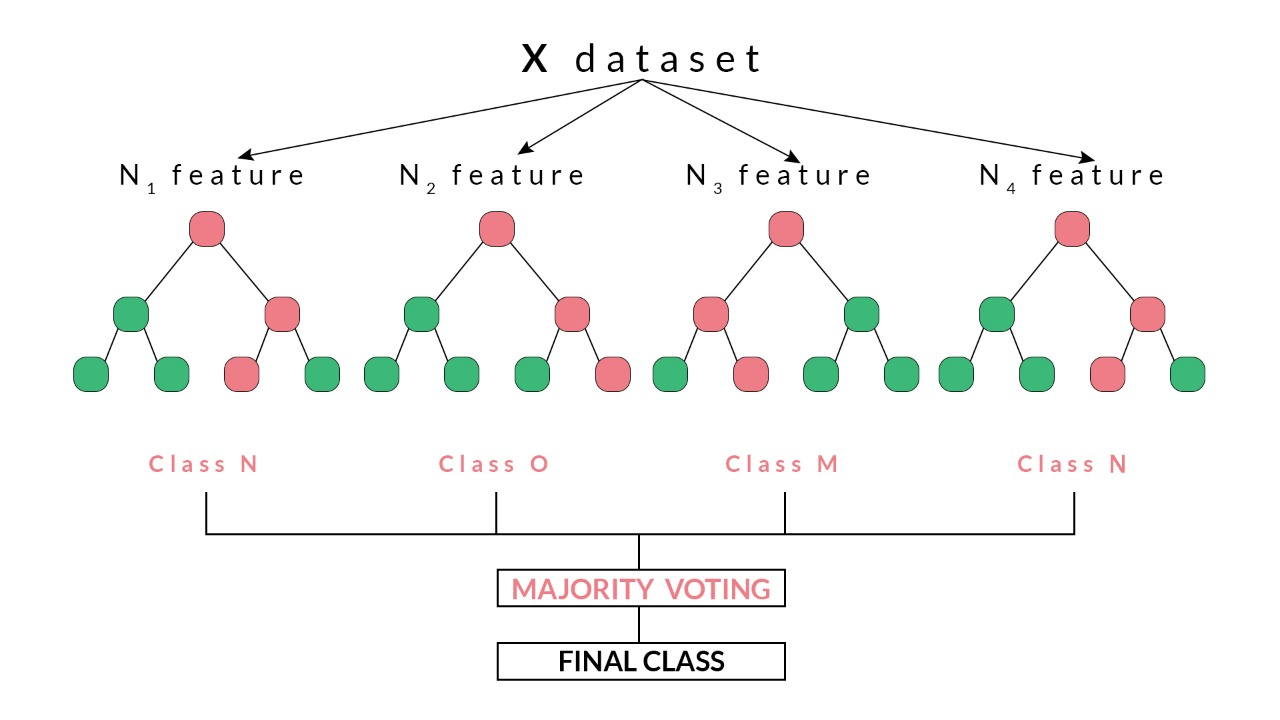
\includegraphics[width=\linewidth]{random-forest.jpeg}
  \caption{Random Forest}
  \label{fig:algo2}
\end{figure}

% You must have at least 2 lines in the paragraph with the drop letter
% (should never be an issue)
\subsection{Methods}
The data visualization method will consist
of different visualization techniques including
bar graphs, histogram, pi chart etc. \\
Now to machine learning model will consist of 2 parts
\begin{itemize}
  \item Dynamic rating system
  \item Predicting the win, draw or loss distribution
\end{itemize}

\begin{enumerate}
  \item \textbf{Dynamic Rating system} \\ A dynamic rating system that provides relative measures of superiority between adversaries
  for each league, and which represents an extended version of the pi-rating system
  (Constantinou and Fenton) which has been proved to be better than the widely accepted
  ELO rating system. In this paper it is considered that a team can participate in different leagues through promotion
  or relegation. Each team has a different rating corresponding to the different leagues
  they are part of. \\
  We will be predicting the player form in the upcoming match
  and using the player form considering over/under performace of
  all the players, a team rating will be generated for that particular
  match.
  \item \textbf{Prediction}
  \begin{enumerate}
    \item \textbf{Support Vector Machine} \\
    Support Vector Machines (SVMs) are Machine Learning models for both classifica-
tion and regression. An SVM model represents the training data as points in space so
that examples falling in different categories are divided by a hyperplane
that is as far as possible from the nearest data point.
Advantages for using Support Vector Machines include that they are effective in highdimensional
spaces, that they are memory efficient thanks to the use of a subset of
training points in the decision function, and finally that they are versatile through
the use of different possible kernel functions. On the other hand, using SVMs can
have some disadvantages: they do not directly provide probability estimates for clas-
sification problems, and correctly optimising the kernel function and regularization
term is essential to avoid overfitting.
    \item \textbf{Neural Networks model} \\
    Neural Networks, also known as Artificial Neural Networks (ANNs), are systems that
are based on a collection of nodes (neurons) that model at an algorithmic level the
links between neurons in the human brain.
Each neuron can receive a signal from neurons and pass it on to other neurons.
Two neurons are connected by an edge which has a weight assigned to it, which
models the importance of this neuron’s input to the other neuron’s output.
    \item \textbf{Bayesian Network model} \\
    Since the aim here is to convert rating discrepancies into match predictions, we
require an input node that takes such rating discrepancies as input, and a latent node that
outputs the posterior probabilities of the 1X2 distribution, given the rating discrepancy input.
  \end{enumerate}
\end{enumerate}

\subsection{Tools used}
Using the API-football API to get the most recent data, fixtures, and player statistics
To train the models, using the Kaggle data set which consists of the data from 1872-2019 for better accuracy of the models.

To implement this project, a web interface which will comprise of the following components will be used:
\begin{itemize}
  \item \textbf{Backend}: (For analysis and to fetch data) \newline
Using \textbf{node.js}
  \item \textbf{Machine Learning}: (To predict the player performance or win percentage) \\ Using 
  \begin{itemize}
    \item Tensor flow
    \item Dynamic ratings
    \item Hybrid Bayesian Networks
    \item Random Forest
    \item Support Vectors Machine
  \end{itemize}
  And then concluding the best algorithm possible for football outcome prediction
  \item \textbf{Frontend}: (For visualization and better user experience) \newline
Using \textbf{react.js} with various visualization libraries like recharts or victory or any other similar library

\end{itemize}


% needed in second column of first page if using \IEEEpubid
%\IEEEpubidadjcol





\section{Conclusion}







\appendices

\section{}



\section*{Acknowledgment}



\ifCLASSOPTIONcaptionsoff
  \newpage
\fi


\begin{thebibliography}{1}

\bibitem{b1} M. Stein, H. Janetzko, T. Schreck and D. A. Keim, "Tackling Similarity Search for Soccer Match Analysis: Multimodal Distance Measure and Interactive Query Definition," in IEEE Computer Graphics and Applications, vol. 39, no. 5, pp. 60-71, 1 Sept.-Oct. 2019.%
\bibitem{b2} Constantinou, A.C. Dolores: a model that predicts football match outcomes from all over the world. Mach Learn 108, 49–75 (2019). https://doi.org/10.1007/s10994-018-5703-7
\bibitem{b3}  Journal of Physics: Conference Series, Volume 1020, 1st International Conference on Computing, Technology, Science and Management in Sports (ICoTSM) 2017 25–27 November 2017, Kuching, Sarawak, Malaysia
\bibitem{b4} Prediction of Attendance Demand in European Football Games: Comparison of ANFIS, Fuzzy Logic, and ANN: (2018) Mehmet Şahin and Rızvan Erol 
\bibitem{b5} Johannes Stübinger, Benedikt Mangold and Julian Knoll. Machine Learning in Football Betting: Prediction of Match Results Based on Player Characteristics in MDPI  19 December 2019 20, 90403 Nürnberg, Germany.
\bibitem{b6} Bunker RP, Fayez F (2017) A machine learning framework for sport result prediction. Appl Comput Inf 15(1):27–33
\bibitem{b7} Pettersson D, Nyquist R (2017) Football match prediction using deep learning and recurrent neural network applications. Dissertation, Chalmers University of Technology
\bibitem{b8} Dwijen Rudrapal, Sasank Boro, Jatin Srivastava, Shyamu Singh (2019) A Deep Learning Approach to Predict Football Match Result
\bibitem{b9} A Football Data visualization: The Belgian First Division, Pieterjan Bartels, Tom De, Buyser, Jannes Van Ussel, Dept. of Computer Science, KU Leuven, Leuven, Belgium
\bibitem{b10} Perin, Charles and Vuillemot, Romain and Stolper, C. and Stasko, J. and Wood, J. and Carpendale, Sheelagh. (2018). State of the Art of Sports Data Visualization. Computer Graphics Forum


\end{thebibliography}
\end{document}


